% Chapter 5

\chapter{Implementation} % Main chapter title
\label{chap:Chapter5}

This chapter is dedicated to explain all the implementation details.

It starts by present the two main components of the developed solution the Explanation API and the Web Application.
After that it will describe how the system was deployed.
Lastly, is presented a resume of the implementation which describes in more detail the implemented use cases, the non-functional requirements and the changes made to the original design.

\section{Explanation API}

The Explanation API is responsible for generating explanations to a given input string.
This API was developed using Flask, a lightweight open-source Python web framework, which is explained in more detail in Chapter~\ref{chap:Chapter2}.

In order to perform its main task, this API has available two approaches that can be used individually or to complement each other.

The first approach will only use web scrapping to generate a list of explanation.
For websites where a single page can be a rich source of information like in Priberam\footnote{https://dicionario.priberam.org/}, this approach can yield good results.

The second approach is a combination of web crawling, web scrapping and text summarization.
For websites where the information is scattered across many pages like Wikipedia\footnote{https://pt.wikipedia.org/}, this approach is ideal.

Both approaches are explained in more detailed in the two following sub-sections.
The approach to be used is set on a configuration file, and should depend on the initial source of information.

(CONFIG FILE CODE) %TODO

For Portuguese, it was used a combination of both approaches.
The first displayed explanation will be generated using the first approach with Priberam\footnote{https://dicionario.priberam.org/} as the source page.
This decision was due to the fact that this page presents precise and simple information and it also divides the page based on the context of a given expression.
The second approach is used when generating an alternative explanation, having Wikipedia as the starting page.
Wikipedia was chosen as the starting page of the second approach due to the fact that it is linked to many other pages which will increase the changes for the text summarization to yield better results.

After having a list of explanations it is necessary to order this list according to the needs of the target audience.
To accomplish this, it was developed a formula that calculates the readability of a sing language sign.
This formula is described in more detail in the following sub-section "LGP Readability Formula".
Note that this was specifically developed for the \gls{LGP} so it it will only be used to for explanations generated in Portuguese.

With a list of explanation sorted, the response object is created.
These response will have the input string, the list of explanation, the source page and a list of links that can provide additional information.
The list of additional information can be preset in a configuration file or generated during the web-crawling phase of the second approach

(RESPONSE OBJECT CODE) %TODO

\subsection{First approach}

These approach was created during the development of the first prototype, also known as Minimum Value Product, that was presented in Chapter~\ref{chap:Chapter3} and consists of a web scrapping process.

It starts by getting the targeted page source code using the Python library Requests\footnote{https://requests.readthedocs.io/en/master/}.
After that, the important text is then filtered form the surrounding noise by exploring the parsed tree with the help of the Beautiful Soup 4 library, which was explained in more detail in Chapter~\ref{chap:Chapter2}.
This extraction process is design for a specific page, so it requires to be recreated if a different page is used.

The following source code is an extract of the web scrapping algorithm design for the Priberam page.

(WS PRIBERAM CODE) %TODO

In the code displayed above is show how it extracts text from the content of a very specific HTML tag.

This process will return a list of expressions per context per explanation.

(RESULT CODE) %TODO

The main advantage of this approach are the following:
\begin{itemize}
        \item Obtaining an initial explanation is very fast since it only extracts the targeted information of a specified page.
\end{itemize}

In regards to disadvantages:
\begin{itemize}
        \item The web scrapping algorithm needs to be specifically developed for the target page.
        \item The text is extracted from a page with content in Portuguese, not \gls{LGP}.
\end{itemize}

\subsection{Second approach}

These approach was created to utilize Information Retrieval, Information Extraction and Text Mining techniques in order to generate an explanation.

It starts by utilizing a web crawler that was created using the Python library Scrapy, which was described in more detail in Chapter~\ref{chap:Chapter2}.
This will crawl the web staring in a predefined page and will download this and all the pages in a crawl depth of 1.
The crawl depth is the level of subpages the web crawler will access that originated from the starting page, it is comparable to folders and their subfolders.
In this case it will only access the subpages of the starting page.

(Spider CODE) %TODO

All the pages are stored locally with their origin link as first line.
This will be latter used to create the API response object.

After the web crawling its time for the web scrapping to extract relevant text from the surrounding noise.
Unlike the web scrapping in the previous approach, this will process multiple pages so it wouldn't be able to target the relevant text.
Thus it will remove the HTML tags, remove the brackets from the text and extra spaces.
The cleared pages are then stored locally.

(HTMLtoTXT CODE) %TODO

The last and most important part of this approach is the text summarization that was created using the Python library NLTK, which was described in more detail in Chapter~\ref{chap:Chapter2}.
Also as mentioned in Chapter~\ref{chap:Chapter2} there are two methods to perform text summarization, extraction and abstraction.
In this approach it was utilized an extractive methodology because it tends to produce summaries specific and not redundant\cite{cheung2008comparing}.

The text summarization process starts by calculate the word frequency of all the words in the content text.
For this it will first tokenize the words of the text and count the number of occurrences of each word, ignoring stop words and punctuation.
Then it will divide the number of occurrences of each words by the number of the most occurring word.

After having the word frequency it will calculate the weighted frequency of each sentence.
To accomplish this, first it will tokenize the content into sentences.
Then it will find the weighted frequency of each sentence by adding the frequency of each word that compose the sentence.

(TEXT SUMMARIZATION CODE) %TODO

The tokenization and the stop words used in this process are built-in functions of the NLTK library.

To finalize this process, it creates a summary using the top seven weighted sentences.
This value may be altered in the summarization configuration.

(RETURN CODE EXAMPLE) %TODO

When this approach is used to generate and alternative explanation which is the case for Portuguese it will take in consideration the context of the previous explanation.
For this, the text summarization will also sort the sentences in crescent order of similarity between the original sentence and each of the sentences of the summary.
The similarity is calculated using the cosine similarity using the following formula:

\begin{equation}
    {similarity(A,B)} = \frac{A \cdot B}{\left \| A \right \| \times \left \| B \right \|}= \frac{\sum_{i=1}^{n} A_{i}B_{i}}{\sqrt{\sum_{i=1}^{n} A_{i}^{2}} \times \sqrt{\sum_{i=1}^{n} B_{i}^{2}}}
\label{similarity}
\end{equation}

The main advantage of this approach are the following:
\begin{itemize}
        \item
\end{itemize}

In regards to disadvantages:
\begin{itemize}
        \item This approach is slower than the first one.
        \item The time it takes to generate an explanation depends on the amount of pages it was to crawl.
        \item
\end{itemize}

\subsection{LGP Readability Formula}

For a regular language, there are metrics, like the readability score, that can be used to classify each expression in order to sort them accordingly.
This score indicates how easily a reader would comprehend the text that he's reading.

There are multiple formulas that could be used for calculating this score in Portuguese, as shown in Chapter~\ref{chap:Chapter2}.
However, there is none for the \gls{LGP}.

When looking at the readability formulas for Portuguese, it is easy to notice that, all of them take in consideration the same variables, which are common in every written text: characters, complex words, syllables, words and sentences.

After analyzing the \gls{LGP} signs, with the goal of creating a new readability calculation formula, all the shared variables where identified:

\begin{itemize}
    \item \textbf{Hand configurations (CF)} - The hand shape in a particular moment.
    \item \textbf{Moments (MT)} - The position of the hand in relation to the body.
    \item \textbf{Hands (HS)} - Both hands or only the dominant hand.
    \item \textbf{Facial expressions (FE)} - Motion or position of the face muscles.
\end{itemize}

Using those variables the following formula was created:

\begin{equation}
(0.7 \times CF + 0.3 \times MT + 1 \times FE) \times (0.5 \times HS)
\label{wordScore}
\end{equation}

This formula was tested using the signs from a local database that had the same values as the avatar database.
The constant values, that were initially set to 1, were manually adjusted to produce a more compact interval of results.
However, the constant value for the facial expressions was unaltered due to the current version of the avatar not supporting them.
In the Table \ref{table:signs} is shown an example of some signs and their readability score.

\begin{table}[H]
    \centering
    \caption{Word readability scores.}
    \label{table:signs}
    \begin{tabular}{l|l|l|l|l}
        {\bfseries Sign} & {\bfseries CF} & {\bfseries MT} & {\bfseries HS} & {\bfseries Score} \\
        \hline
        Javali & 1 & 1 & 1 & 1.00  \\
        \hline
        Fornecedor & 2 & 6 & 1 & 2.09  \\
        \hline
        Auxílio & 2 & 4 & 2 & 3.59 \\
        \hline
        Consumo & 4 & 6 & 2 & 5.60 \\
        \hline
        Esclarecer & 7 & 7 & 2 & 8.00 \\
    \end{tabular}
\end{table}

In order to calculate the score of an entire sentence, the sum of the scores of each word were divided by the number of words in the sentence, creating the following formula:

\begin{equation}
    \frac{(0.7 \times CF + 0.3 \times MT + 1 \times FE) \times (0.5 \times HS)}{WO}
\label{sentenceScore}
\end{equation}

This formula is used to calculate the readability score of the generated explanations.
In the Table~\ref{table:sentences} is shown an example of some sentences and their readability score.

%TODO fix table
\begin{table}[H]
    \centering
    \caption{Sentence readability scores.}
    \label{table:sentences}
    \begin{tabular}{l|l}
        {\bfseries Sentence} & {\bfseries Score} \\
        \hline
        s1 & 1  \\
        \hline
        s2 & 2  \\
        \hline
        s3 & 2 \\
        \hline
        s4 & 4 \\
        \hline
        s5 & 7 \\
    \end{tabular}
\end{table}

\section{Web Application}

A user interacts with the web application that was developed in React, an open-source JavaScript framework for building user interfaces.
Here, the user can search for the desired concept, as well as changing the page language.
This is also the place where the generated explanations are shown in plain text and in \gls{LGP} by the avatar.
After each explanation, it is also presented their \gls{LGP} Readability Score, which is presented more in depth in the following subsection, as well as feedback options.
If one of the presented explanations is not acceptable, it is possible for the user to request a new one.

\begin{itemize}
    \item \textbf{App}
    \item \textbf{Avatar}
    \item \textbf{Display}
    \item \textbf{Navbar}
    \item \textbf{Search}
\end{itemize}

\dots %TODO Ideoma

\dots %TODO mencionar que foi estruturado para ser responsive apesar de não ser necessariamete um requisito

\section{Hosting}

reverse proxy

pm2 react service

systemctl flask service

certbot https

\dots %TODO

\section{Resume}

\dots %TODO

\subsection{Logic view}

\begin{figure}[H]
\centering
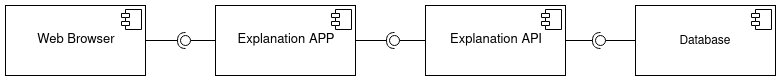
\includegraphics[width=\textwidth,keepaspectratio]{ch5/assets/component_diagram_Implement.png}
\caption[Component Diagram Implementation]{Component Diagram Implementation}
\label{fig:componentImp}
\end{figure}

\dots

\subsection{Use cases}

In this section the use cases are presented to better understand how the designed requirements were implemented.

\dots %TODO

\subsubsection{US01: Find explanation}

\begin{figure}[H]
\centering
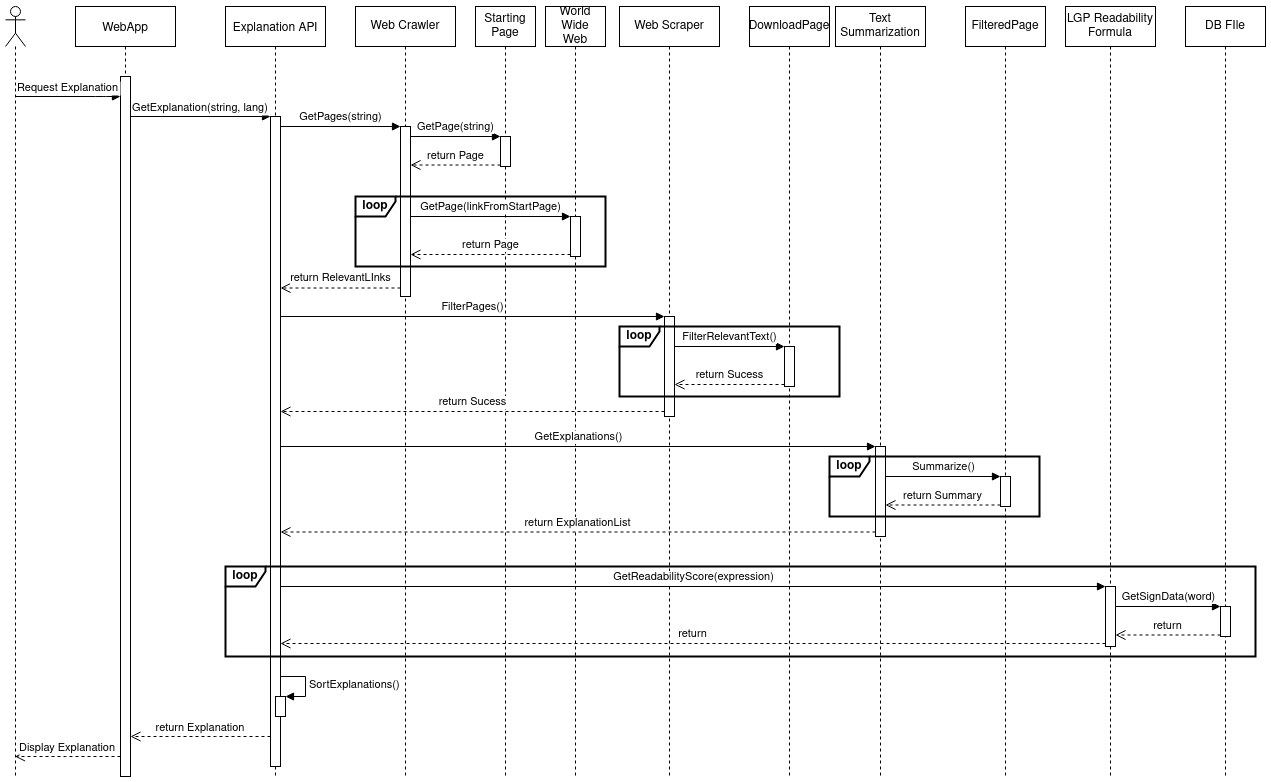
\includegraphics[width=\textwidth,keepaspectratio]{ch5/assets/US01_SD_Implement.png}
\caption[Sequence Diagram Implementation US01]{Sequence Diagram - Implementation US01}
\label{fig:uc01Imp}
\end{figure}

\dots %TODO

\subsubsection{US02: Obtain alternative explanation}

\begin{figure}[H]
\centering
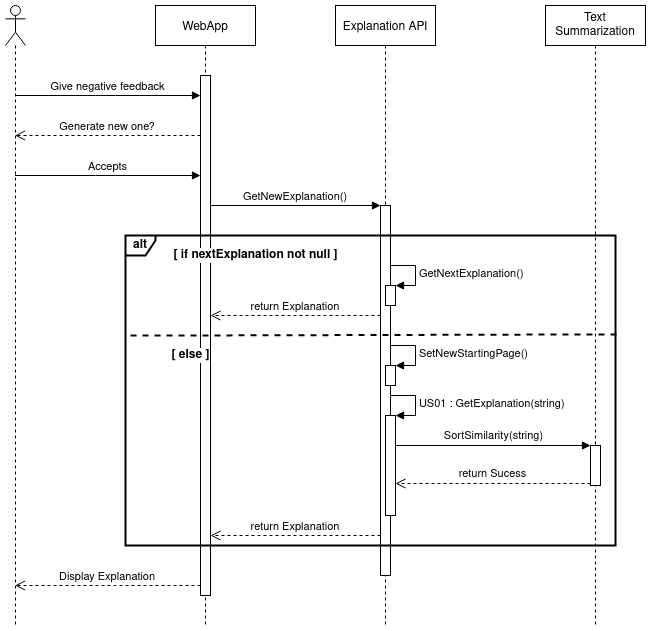
\includegraphics[scale=0.45]{ch5/assets/US02_SD_Implement.png}
\caption[Sequence Diagram Implementation US02]{Sequence Diagram - Implementation US02}
\label{fig:uc02Imp}
\end{figure}

\dots %TODO

\subsubsection{US04: Change language}

\begin{figure}[H]
\centering
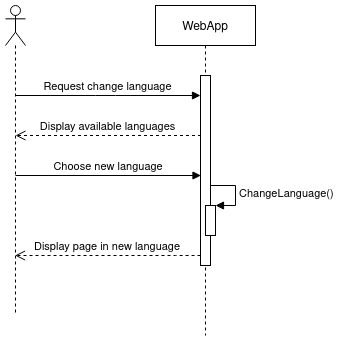
\includegraphics[scale=0.45]{ch5/assets/US04_SD_Implement.png}
\caption[Sequence Diagram Implementation US04]{Sequence Diagram - Implementation US04}
\label{fig:uc04Imp}
\end{figure}

\dots %TODO

\subsection{Non-Functional Requirements}

\dots %TODO

\subsection{Deployment view}

\begin{figure}[H]
\centering
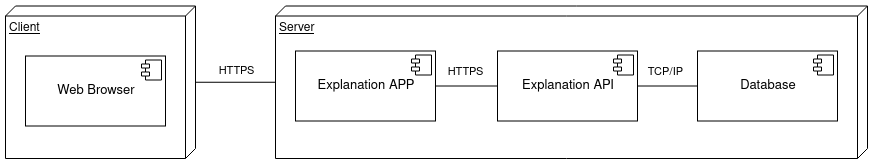
\includegraphics[width=\textwidth,keepaspectratio]{ch5/assets/deployment_diagram_Implement.png}
\caption[Deployment Diagram Implementation]{Deployment Diagram Implementation}
\label{fig:deployImp}
\end{figure}

\dots %TODO
